%%%%%%%%%%%%%%%%%
%BEGIN          %
%%%%%%%%%%%%%%%%%
%%%%%%%%%%%%%%%%%%%%%%%%%
% PACKAGES              %
%%%%%%%%%%%%%%%%%%%%%%%%%
\documentclass{report}
\usepackage[utf8x]{inputenc}  % accents
\usepackage{geometry}         % marges
\usepackage[francais]{babel}  % langue
\usepackage{graphicx}         % images
\usepackage{verbatim}         % texte préformaté
\usepackage{fancyhdr}         % fancy






% Titre de ce fichier dans le fancy 
\newcommand{\titre}{{\Huge Manuel Aide}\\Groupe B}
\newcommand{\titrehead}{Aide}
%%%%%%%%%%%%%%%%%%%%%%%%%
% PRÉAMBULE             %
%%%%%%%%%%%%%%%%%%%%%%%%%
\title{\titre{}}
\author{}
% laisser vide pour date de compilation
\date{} 

% FORMAT PAGES         
\pagestyle{fancy} % nom du rendu (définit les lignes suivantes)
        \lhead{} % left head
        \chead{\titrehead{}} % center head
        \rhead{} % right head
        \lfoot{} % left foot
        \cfoot{\thepage} % center foot
        \rfoot{} % right foot


% Ce fichier est un préambule commun à toutes les sources LaTeX.
% Il est inclus par toutes les sources et permet d'avoir un formatage commun facilement modifiable.




\begin{document}


\chapter{Liste des aides disponible}


\section{Les cases faciles à noircir}
	\paragraph{}
	\begin{itemize}
		\item Si une grille est de taille 10x10 et que sur une ligne(ou une colonne) est indiqué 10, c'est à dire que toutes les cases de la ligne ou de la colonne doivent être noirci.\\

	\begin{center}
		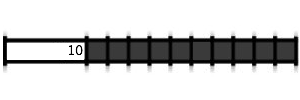
\includegraphics{data/manuels/10par10.png}\\
	\end{center}

		\item Si une ligne (ou une colonne) à sa première(ou dernière) case de noircie et que le premier chiffre de cette ligne est 3, vous pouvez noircir les deux cases suivantes(resp. précédentes). En effet le 3 correspond obligatoirement aux trois première cases de la ligne.\\
	\begin{center}
		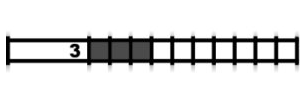
\includegraphics{data/manuels/3premier.png}\\
	\end{center}
\newpage
		\item Si une ligne(ou une colonne) comporte 10 cases et que seules 7 cases sont à noircir, vous pouvez noircir les quatres cases centrales : ces cases seront noircies quelque soit la solution de cette ligne (ou de cette colonne). Cette astuce fonctionne dès qu'une ligne ou un colonne ne possède qu'un nombre et que ce nombre est strictement plus grand que la moitié des cases de cette ligne ou de cette colonne.\\

	\begin{center}
		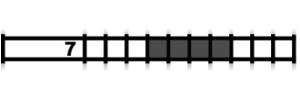
\includegraphics{data/manuels/7casesSur10.png}
	\end{center}
		
		\item Si la somme des chiffres et des intervalles (au minimum 1 intervalle entre deux chiffres) d'une ligne(ou d'une colonne) est égale à la longueur de la ligne(ou de la colonne), vous pouvez noircir les cases dans l'ordre des chiffres. Par exemple sur une grille 10x10, si une ligne à comme chiffre 5 et 4, la somme est bien égale a 10(5+1+4) donc vous pouvez noircir les 5 premières et les 4 dernières en laissant une case qui sera coché entre.\\
		
	\begin{center}
		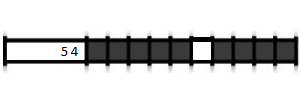
\includegraphics{data/manuels/sommeChiffreInterv.png}
	\end{center}
	
	
	\end{itemize}

\section{Les cases à éliminer}
	\paragraph{}
	\begin{itemize}
		\item Vous pouvez aussi éliminer les cases qui ne sont évidemment pas à noircir en les marquant d'une croix(click droit), cela permet de voir plus clair dans la résolution du picross. Par exemple si une ligne contient trois cases à noircir et que vous avez déjà noircies ces trois cases, vous pouvez éliminer toutes les autres cases de cette ligne.
	\end{itemize}
\end{document}
